% Chapter Template


\chapter{Experiments} % Main chapter title

\label{Experiments} % Change X to a consecutive number; for referencing this chapter elsewhere, use \ref{ChapterX}

%----------------------------------------------------------------------------------------
%	SECTION 1
%----------------------------------------------------------------------------------------
\begin{figure}[H]
    \centering
    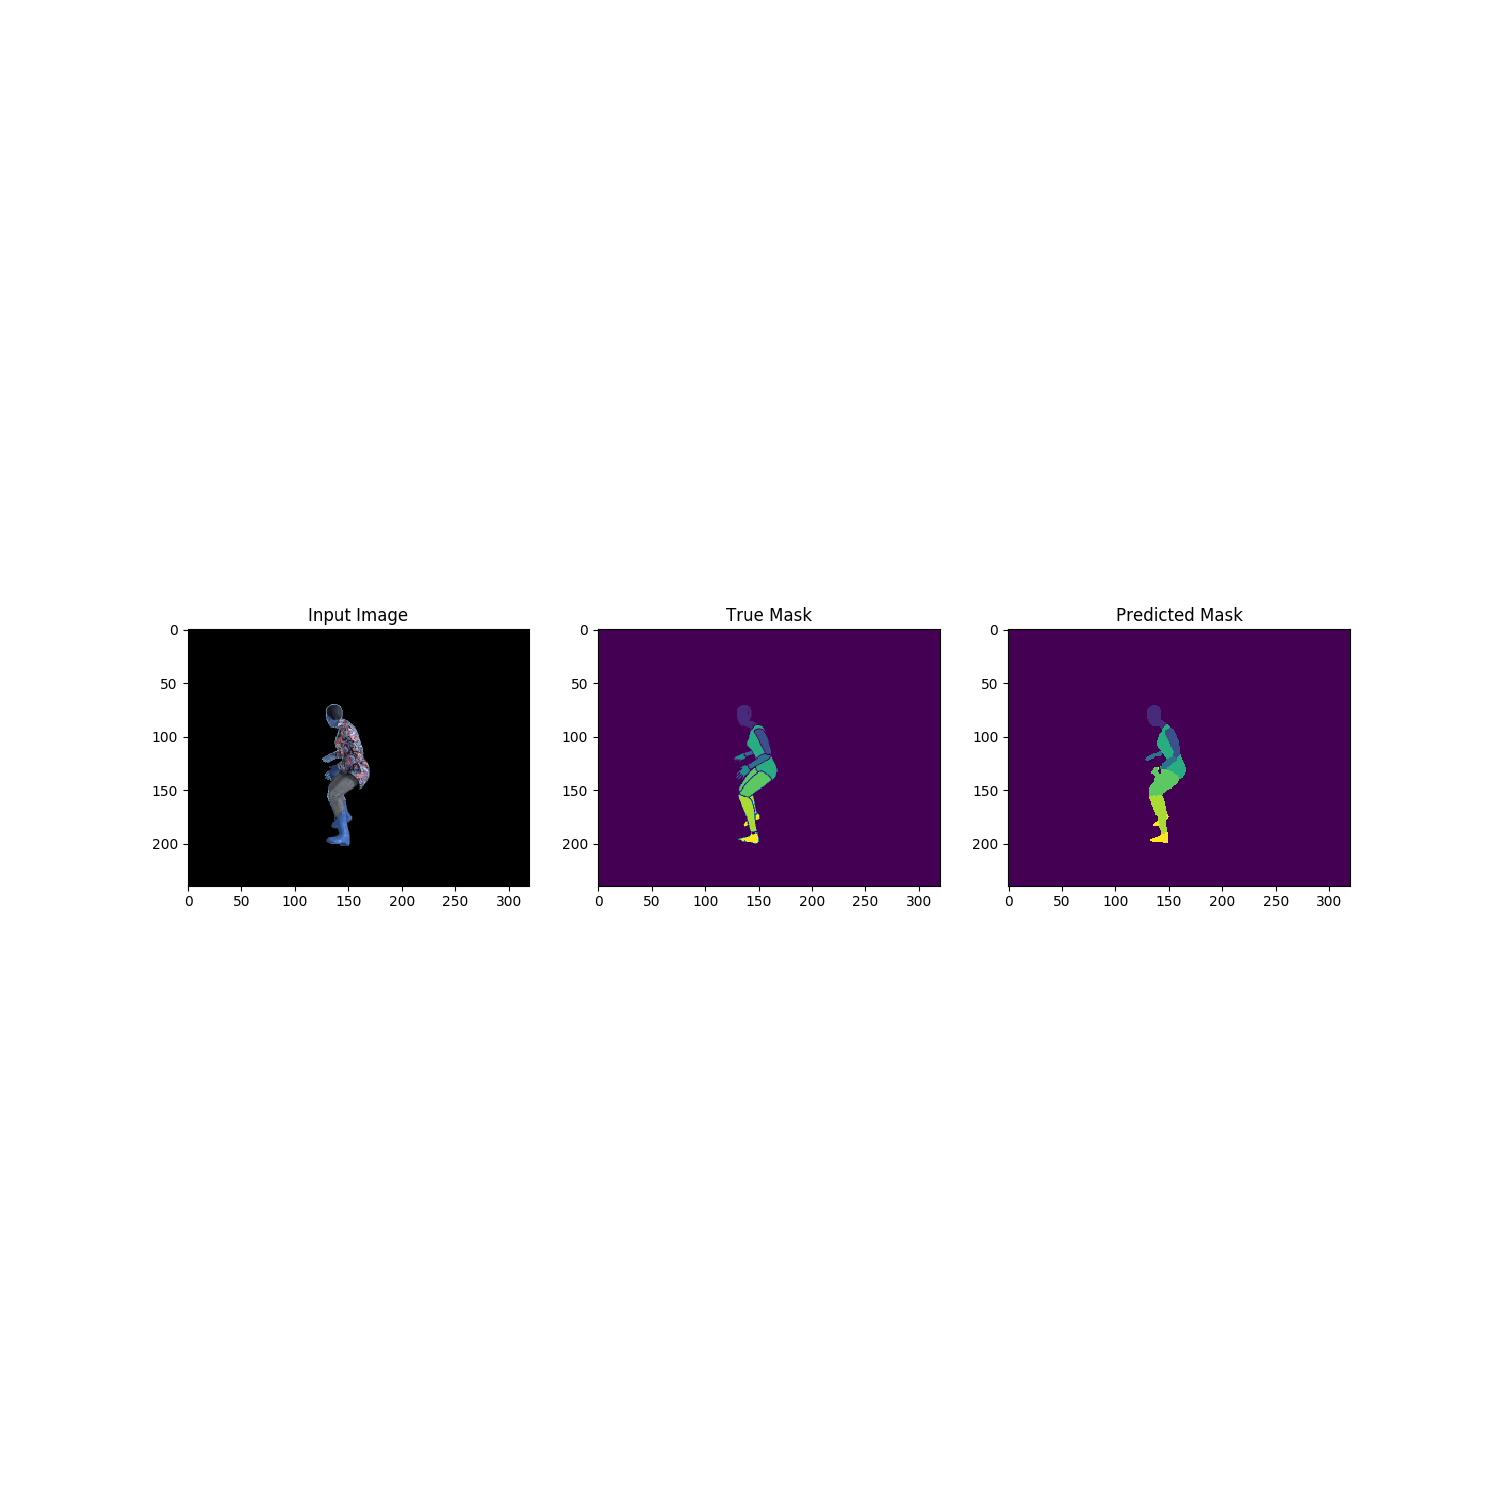
\includegraphics[width=\textwidth, height=\textheight, keepaspectratio]{img/adam_prediction_3845_train.png}
    \decoRule
    \caption[Predicted Mask]{Predicted mask after 3845th epoch with custom loss function and Adam optimizer\_kps}
    \label{fig:adam-prediction}
\end{figure}
% with custom loss function and Adam optimizer_kps


%\section{Different Net Architectures}
\section{Ablation Study}


%-----------------------------------
%	SUBSECTION 1
%-----------------------------------
\subsection{Body Parts Module }
\label{RBP}


\paragraph{Stride-down, -up convolution before \gls{bl}}

\paragraph{MobileNet extended with UNet}
\paragraph{MobileNet extended with HRNet}

\paragraph{Experiment with concat and add layers}

\paragraph{Best performing network HRNet v7}

\begin{figure}[H]
    \centering
    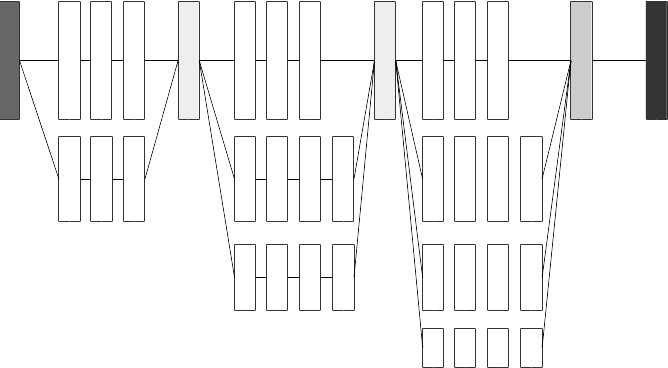
\includegraphics[width=\textwidth,height=\textheight,keepaspectratio]{img/network_v7_hrnet.png}
    \decoRule
    \caption[HRNet v7]{HRNet v7.}
    \label{fig:hrnet-v7}
\end{figure}


%-----------------------------------
%	SUBSECTION 2
%-----------------------------------
\subsection{Joint Module }

\paragraph{Dense Modules}
\paragraph{Fully Convolutional}

%-----------------------------------
%	SECTION 2
%-----------------------------------
\section{Comparison of Optimizer Algorithms}

\begin{itemize}
    \item Adam
    \item Nadam
    \item SGD
    \subitem constant learning rate
    \subitem Constant decreasing learning rate
    \subitem Constant decreasing learning rate with reset of learning rate on plateau
    \subitem Increasing decreasing learning rate on plateau
\end{itemize}

\paragraph{Comparison of Adam, Nadam and SGD}
\begin{figure}[H]
    \centering
    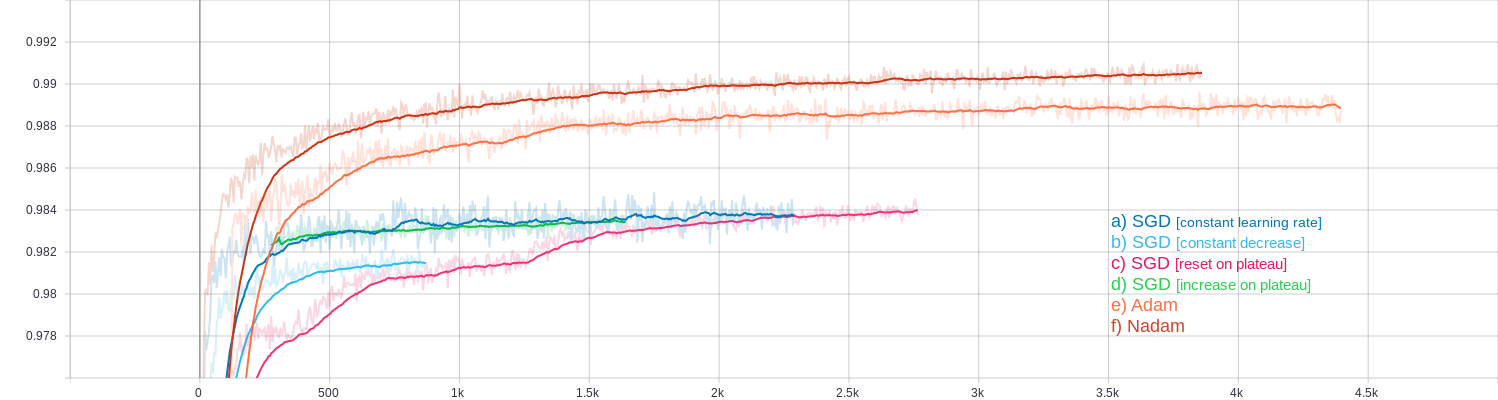
\includegraphics[width=\textwidth,height=\textheight,keepaspectratio]{img/accuracy_all.png}
    \decoRule
    \caption[Accuracy]{Accuracy}
    \label{fig:accuracy}
\end{figure}
\begin{figure}[H]
    \centering
    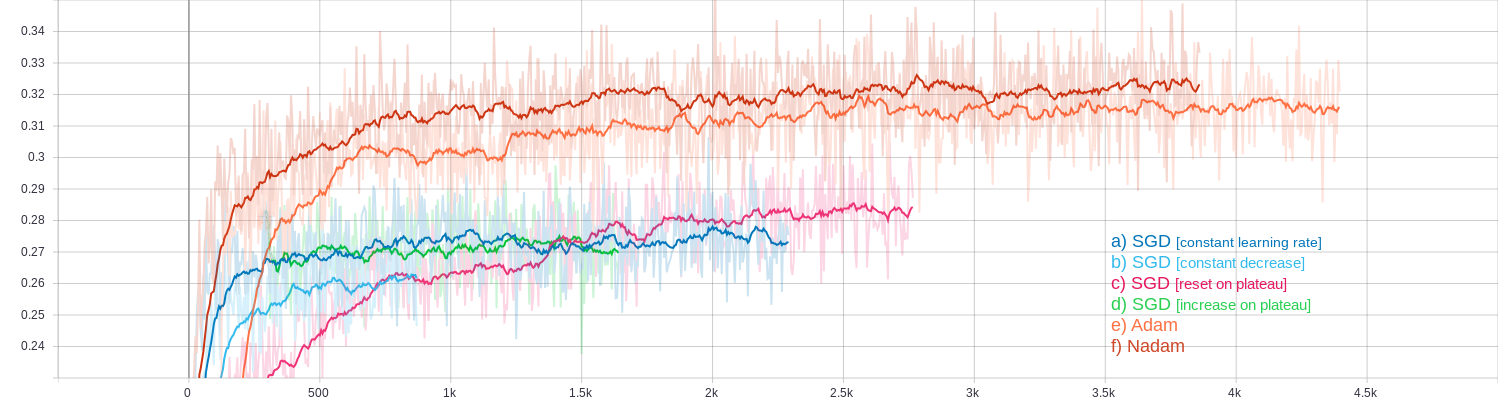
\includegraphics[width=\textwidth,height=\textheight,keepaspectratio]{img/accuracy_body_part_all.png}
    \decoRule
    \caption[Correct BPR]{Correct body part pixel relation}
    \label{fig:acc-bp}
\end{figure}
\begin{figure}[H]
    \centering
    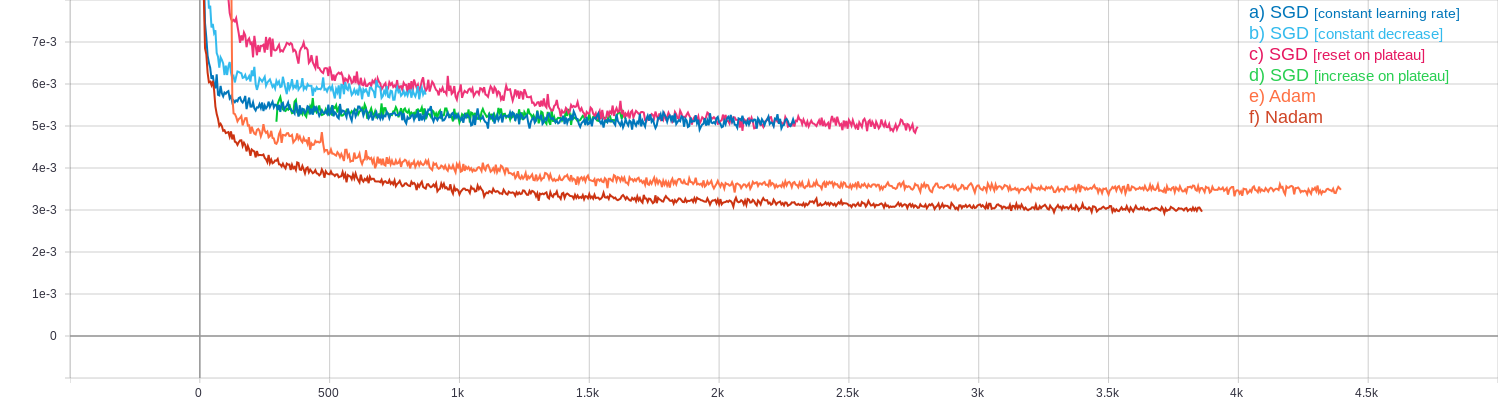
\includegraphics[width=\textwidth,height=\textheight,keepaspectratio]{img/loss_all.png}
    \decoRule
    \caption[loss]{Loss}
    \label{fig:loss}
\end{figure}

\paragraph{Experiments with SGD}
\begin{figure}[H]
    \centering
    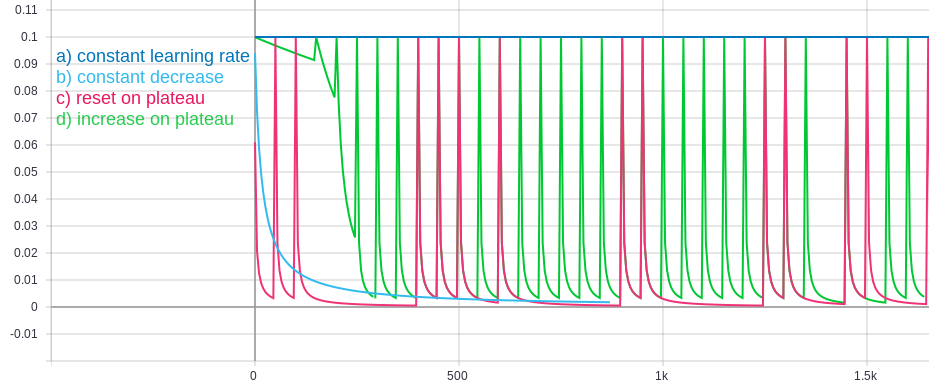
\includegraphics[width=\textwidth,height=\textheight,keepaspectratio]{img/learning_rate2.png}
    \decoRule
    \caption[Learning Rate SGD]{Learning Rate SGD.}
    \label{fig:sgd-learning-rate}
\end{figure}

\begin{figure}[H]
    \centering
    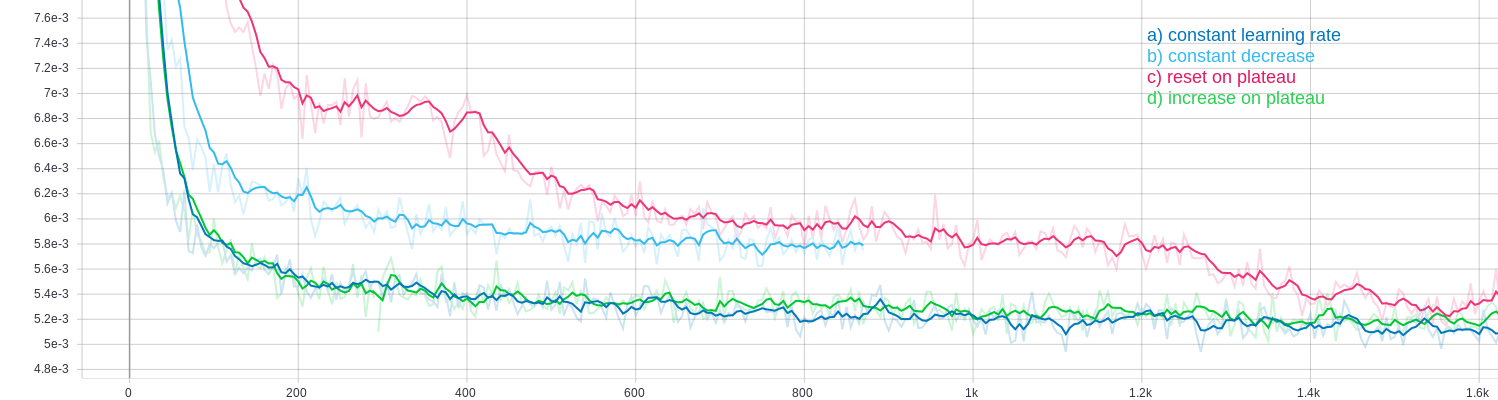
\includegraphics[width=\textwidth,height=\textheight,keepaspectratio]{img/loss_sgd.png}
    \decoRule
    \caption[Loss SGD]{Loss SGD.}
    \label{fig:sgd-loss}
\end{figure}

\begin{figure}[H]
    \centering
    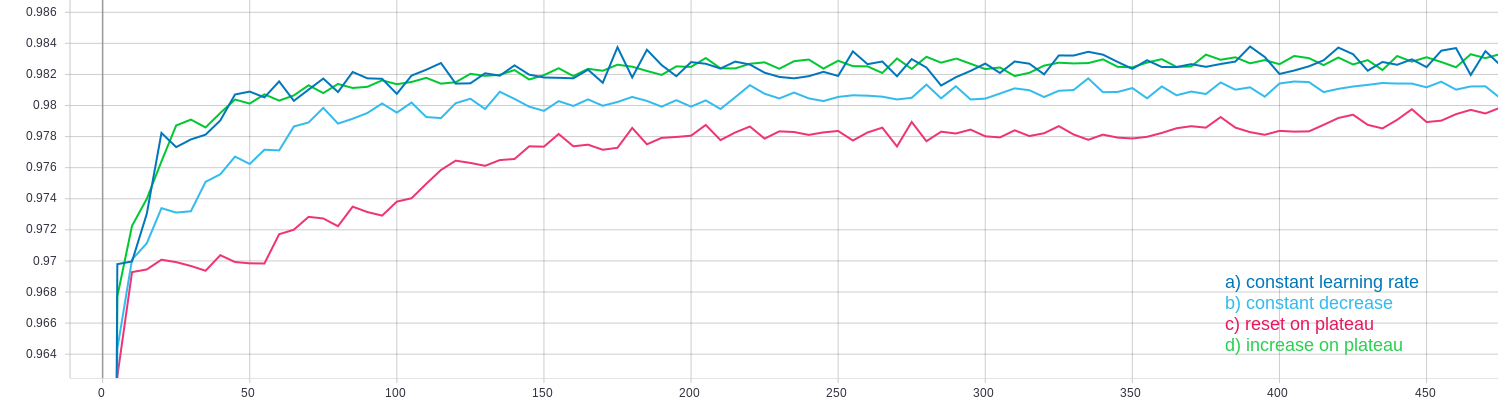
\includegraphics[width=\textwidth,height=\textheight,keepaspectratio]{img/accuracy_sgd.png}
    \decoRule
    \caption[Accuracy SGD]{Accuracy SGD.}
    \label{fig:sgd-accuracy}
\end{figure}

%----------------------------------------------------------------------------------------
%	SECTION 3
%----------------------------------------------------------------------------------------


\section{Performance of loss functions}
All performance measures are conducted on the Nadam optimizer\_kps with the HRNet for body part recognition from
Recognition of body parts \ref{RBP}

\subsection{Sparse Categorical Cross Entropy}

\subsection{Mean Squared Error}

\subsection{Our custom loss function CILoss}
This loss function confronts the problem of class imbalance, which especially occurs in body part recognition.
The background pixels appear most often, and the different body part classes occur by far less often and event they
differentiate a lot in their relative occurrence.

We try to confront this problem with a weighed map, which takes the body parts as a graph and calculates
the distances from each body part $b_x$ to all other body parts $b_n$, and stores this data inside a table.

Additionally this weight map is evened out with a multiplier to reduce the distances and facilitate
the learning process for the network.

$$\theta=y_t(x)-y_p(x)$$
$$\delta=\theta*\mu[argmax(y_t)] $$
$$L=\sum_{i=0}^{n}\theta_i+\delta_i$$


\begin{figure}[H]
    \centering
    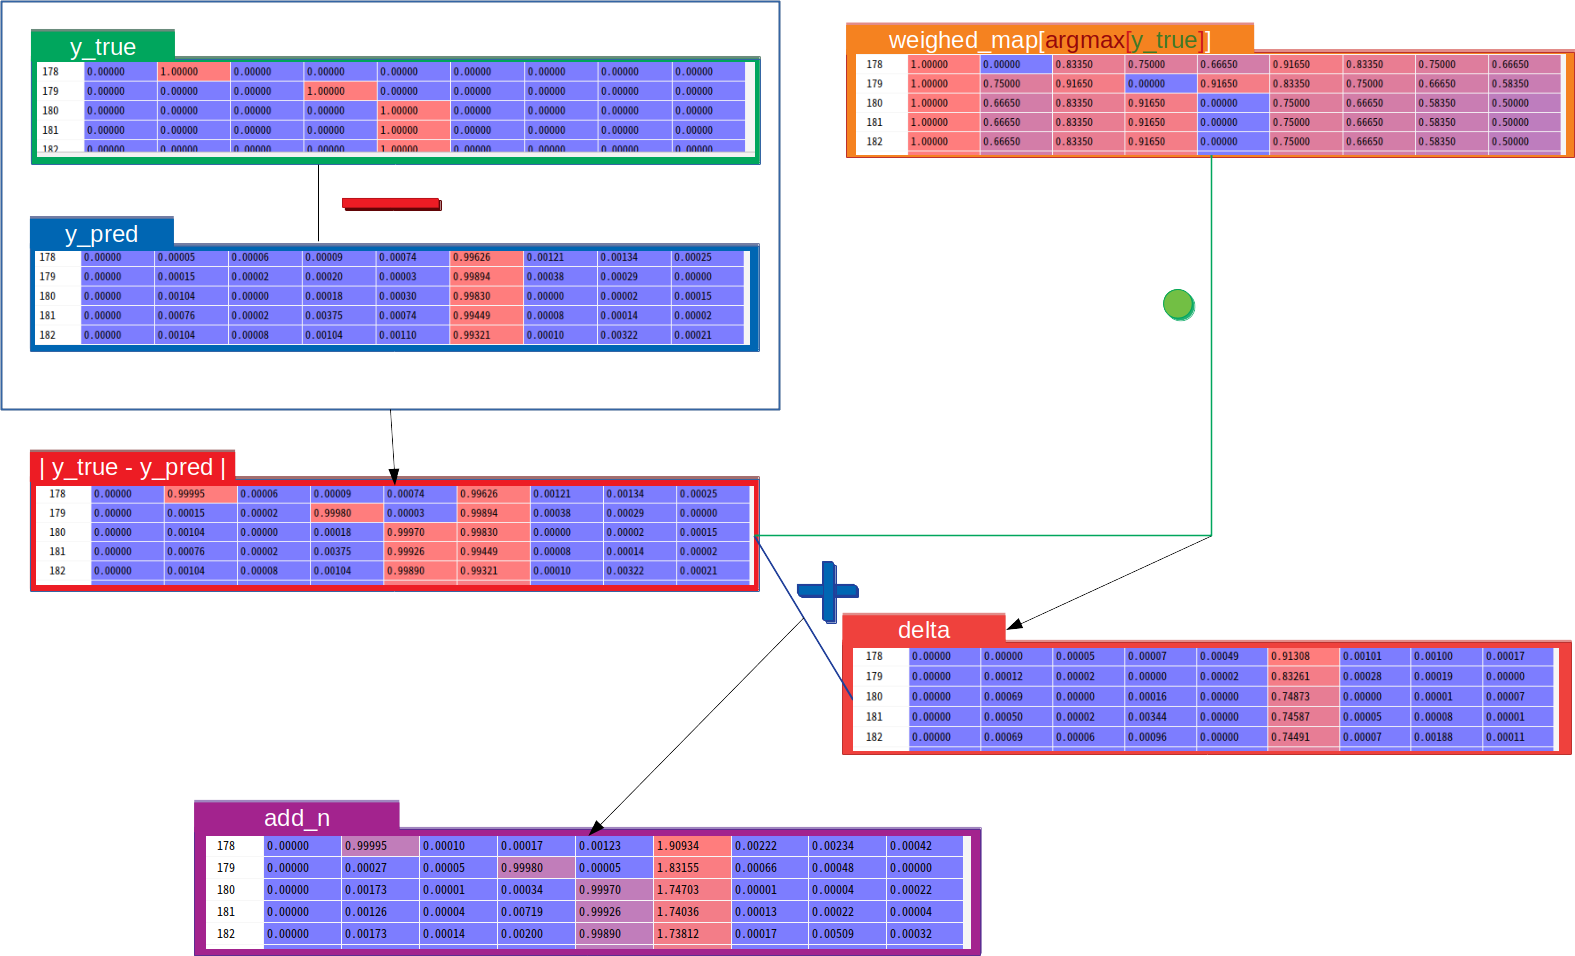
\includegraphics[width=\textwidth,height=\textheight,keepaspectratio]{img/loss_calculation.png}
    \decoRule
    \caption[CILoss]{Visualization of custom loss calculation}
    \label{fig:ciloss-calc}
\end{figure}
